%%
%% ASE 2026 paper, ACM sigconf template
%%
\documentclass[sigconf]{acmart}

%% Packages
\usepackage{algorithmic}
\usepackage{graphicx}
\usepackage{textcomp}
\usepackage{xcolor}
\usepackage{enumitem}
\usepackage{multirow}
\usepackage{tabularx}
\usepackage{array}
\usepackage{booktabs}
\usepackage{siunitx}
\usepackage{subcaption}
\usepackage{adjustbox}
\usepackage{dblfloatfix}

%% \BibTeX command to typeset BibTeX logo in the docs
\AtBeginDocument{%
  \providecommand\BibTeX{{%
    Bib\TeX}}}

%% Suppress copyright/reference blocks for submission stage
\setcopyright{none}
\settopmatter{printacmref=false}
\renewcommand\footnotetextcopyrightpermission[1]{}
\pagestyle{plain}

%%
%% The document starts here
%%
\begin{document}

%%
%% Title and author information
%%
\title{Root Cause Analysis for RISC-V Build Failures: From Long-Range Log Compression to Traceable Rule Learning}

%% ---- Authors ----
\author{Zehua Wang}
\affiliation{%
  \institution{Institute of Software, Chinese Academy of Sciences}
  \city{Beijing}\country{China}}
\email{wangzehua23@otcaix.iscas.ac.cn}

\author{Zhirou Ma}
\affiliation{%
  \institution{Institute of Software, Chinese Academy of Sciences}
  \city{Beijing}\country{China}}
\email{mazhirou@otcaix.iscas.ac.cn}

\author{Jie Liu}
\authornote{Corresponding author}
\affiliation{%
  \institution{Institute of Software, Chinese Academy of Sciences}
  \city{Beijing}\country{China}}
\email{ljie@otcaix.iscas.ac.cn}

\author{Liangyi Kang}
\affiliation{%
  \institution{Institute of Software, Chinese Academy of Sciences}
  \city{Beijing}\country{China}}
\email{kangliangyi15@otcaix.iscas.ac.cn}

\author{Shuai Wang}
\affiliation{%
  \institution{Institute of Software, Chinese Academy of Sciences}
  \city{Beijing}\country{China}}
\email{wangshuai@otcaix.iscas.ac.cn}

\author{Dan Ye}
\authornote{Corresponding author}
\affiliation{%
  \institution{Institute of Software, Chinese Academy of Sciences}
  \city{Beijing}\country{China}}
\email{yedan@otcaix.iscas.ac.cn}

\author{Jiaxin Zhu}
\affiliation{%
  \institution{Institute of Software, Chinese Academy of Sciences}
  \city{Beijing}\country{China}}
\email{zhujiaxin@otcaix.iscas.ac.cn}

\author{Wei Wang}
\affiliation{%
  \institution{Institute of Software, Chinese Academy of Sciences}
  \city{Beijing}\country{China}}
\email{wangwei@otcaix.iscas.ac.cn}

\author{Hua Zhong}
\affiliation{%
  \institution{Institute of Software, Chinese Academy of Sciences}
  \city{Beijing}\country{China}}
\email{zhonghua@otcaix.iscas.ac.cn}

\renewcommand{\shortauthors}{Wang et al.}

%% Funding acknowledgments (hidden for submission)
%\thanks{Supported by Strategic Priority Research Program of the Chinese Academy of Sciences (XDA0320102), the National Natural Science Foundation of China (42361144884)}

%% Conference information
\acmConference[ASE '26]{2026 41st IEEE/ACM International Conference on Automated Software Engineering}{October 12--16, 2026}{Munich, Germany}
\acmYear{2026}

%%
%% Abstract
%%
\begin{abstract}
Porting open-source software to RISC-V frequently triggers build failures whose root causes are notoriously difficult to diagnose automatically. Build logs routinely span tens of thousands of lines, yet failure-relevant clues constitute fewer than 5\% of the content, and the true root cause often resides hundreds of lines before the terminal error, forming long-range causal dependencies that naive local windowing inevitably misses. Meanwhile, historical repair knowledge is scattered across heterogeneous commits and issues; superficially similar error messages can require entirely different fixes depending on build stage, dependency version, and toolchain context, making similarity-based retrieval prone to misleading recommendations. We propose a two-stage framework addressing both challenges. Multi-Granularity Semantic Compression (MGSC) anchors on explicit errors, backtracks long-range causal entities, and performs lightweight semantic compression to preserve high-fidelity evidence chains within a strict token budget. Historical Rule Learning for Root Cause Analysis (HRL-RCA) distills structured repair rules from historical commits, organizes them into a rule-tree index by error type and build stage, and performs conditional routing with ReAct-style reasoning to generate traceable, evidence-bound diagnoses. On 174 real RISC-V build failures from a production OBS environment, HRL-RCA achieves a composite diagnostic score of 79.0\%, outperforming all baselines, while reducing processing time by 61\% relative to search-based methods.
\end{abstract}

%%
%% Keywords
%%
\keywords{RISC-V, build failure, root cause analysis, log compression, large language model}

%% CCS Concepts (required by ACM)
\begin{CCSXML}
<ccs2012>
<concept>
<concept_id>10011007.10011074.10011099.10011102.10011103</concept_id>
<concept_desc>Software and its engineering~Software testing and debugging</concept_desc>
<concept_significance>500</concept_significance>
</concept>
<concept>
<concept_id>10011007.10011074.10011099.10011102.10011104</concept_id>
<concept_desc>Software and its engineering~Software maintenance tools</concept_desc>
<concept_significance>300</concept_significance>
</concept>
</ccs2012>
\end{CCSXML}

\ccsdesc[500]{Software and its engineering~Software testing and debugging}
\ccsdesc[300]{Software and its engineering~Software maintenance tools}

%%
%% Make title
%%
\maketitle

%% ===== Section 1 Introduction =====
\section{Introduction}

RISC-V has gained significant momentum in recent years, driven by its open instruction-set architecture, modularity, and extensibility~\cite{cui2023risc}, positioning it as a compelling alternative for next-generation general-purpose and domain-specific computing. Sustained investment from both industry and academia has accelerated the porting of mainstream open-source software to RISC-V~\cite{mezger2022survey}. However, upstream codebases have historically been developed and optimized for x86 and ARM, and their ongoing evolution continually introduces architecture-specific features. Consequently, packages previously adapted for RISC-V frequently regress into build failures upon incorporating upstream updates~\cite{lou2020understanding}.

\begin{figure*}[!tb]
    \centering
    \begin{subfigure}[t]{0.48\textwidth}
        \centering
        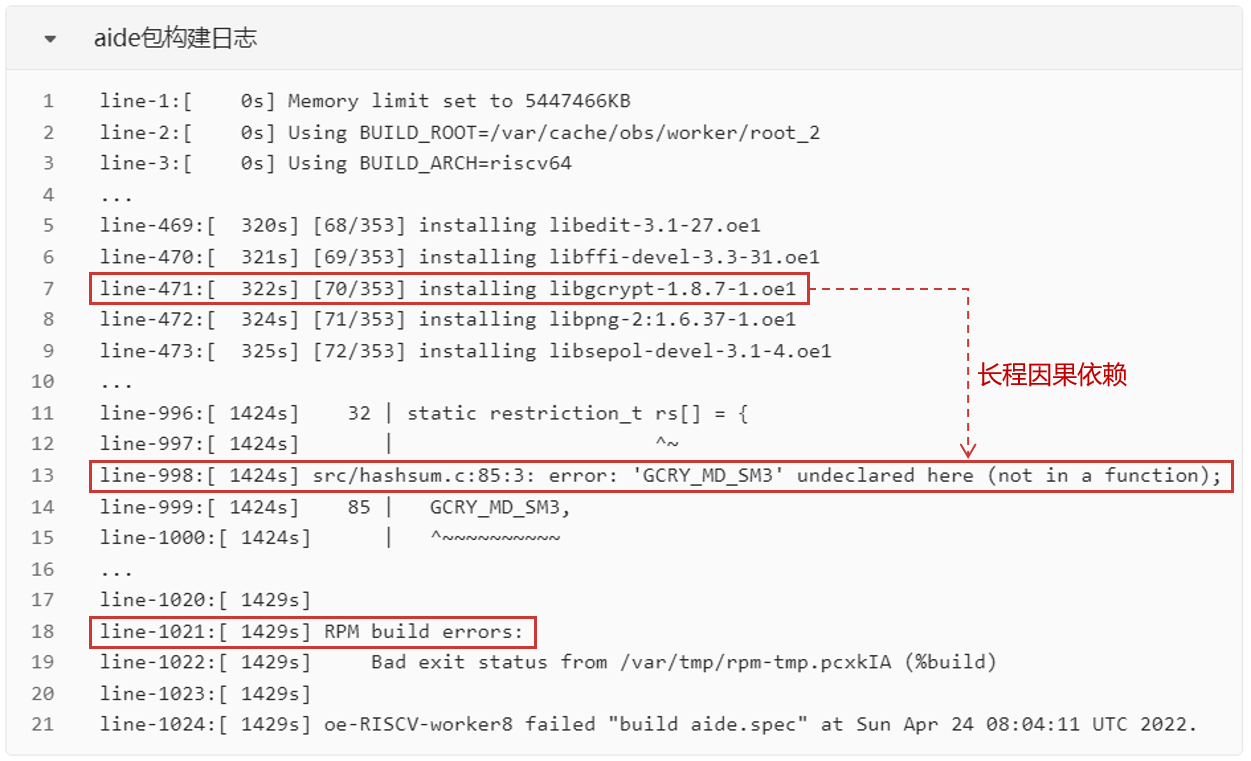
\includegraphics[width=\textwidth]{pic/log-causal-dependency.png}
        \caption{Long-range causal dependencies in build logs}
        \label{fig:causal-dep}
    \end{subfigure}
    \hfill
    \begin{subfigure}[t]{0.48\textwidth}
        \centering
        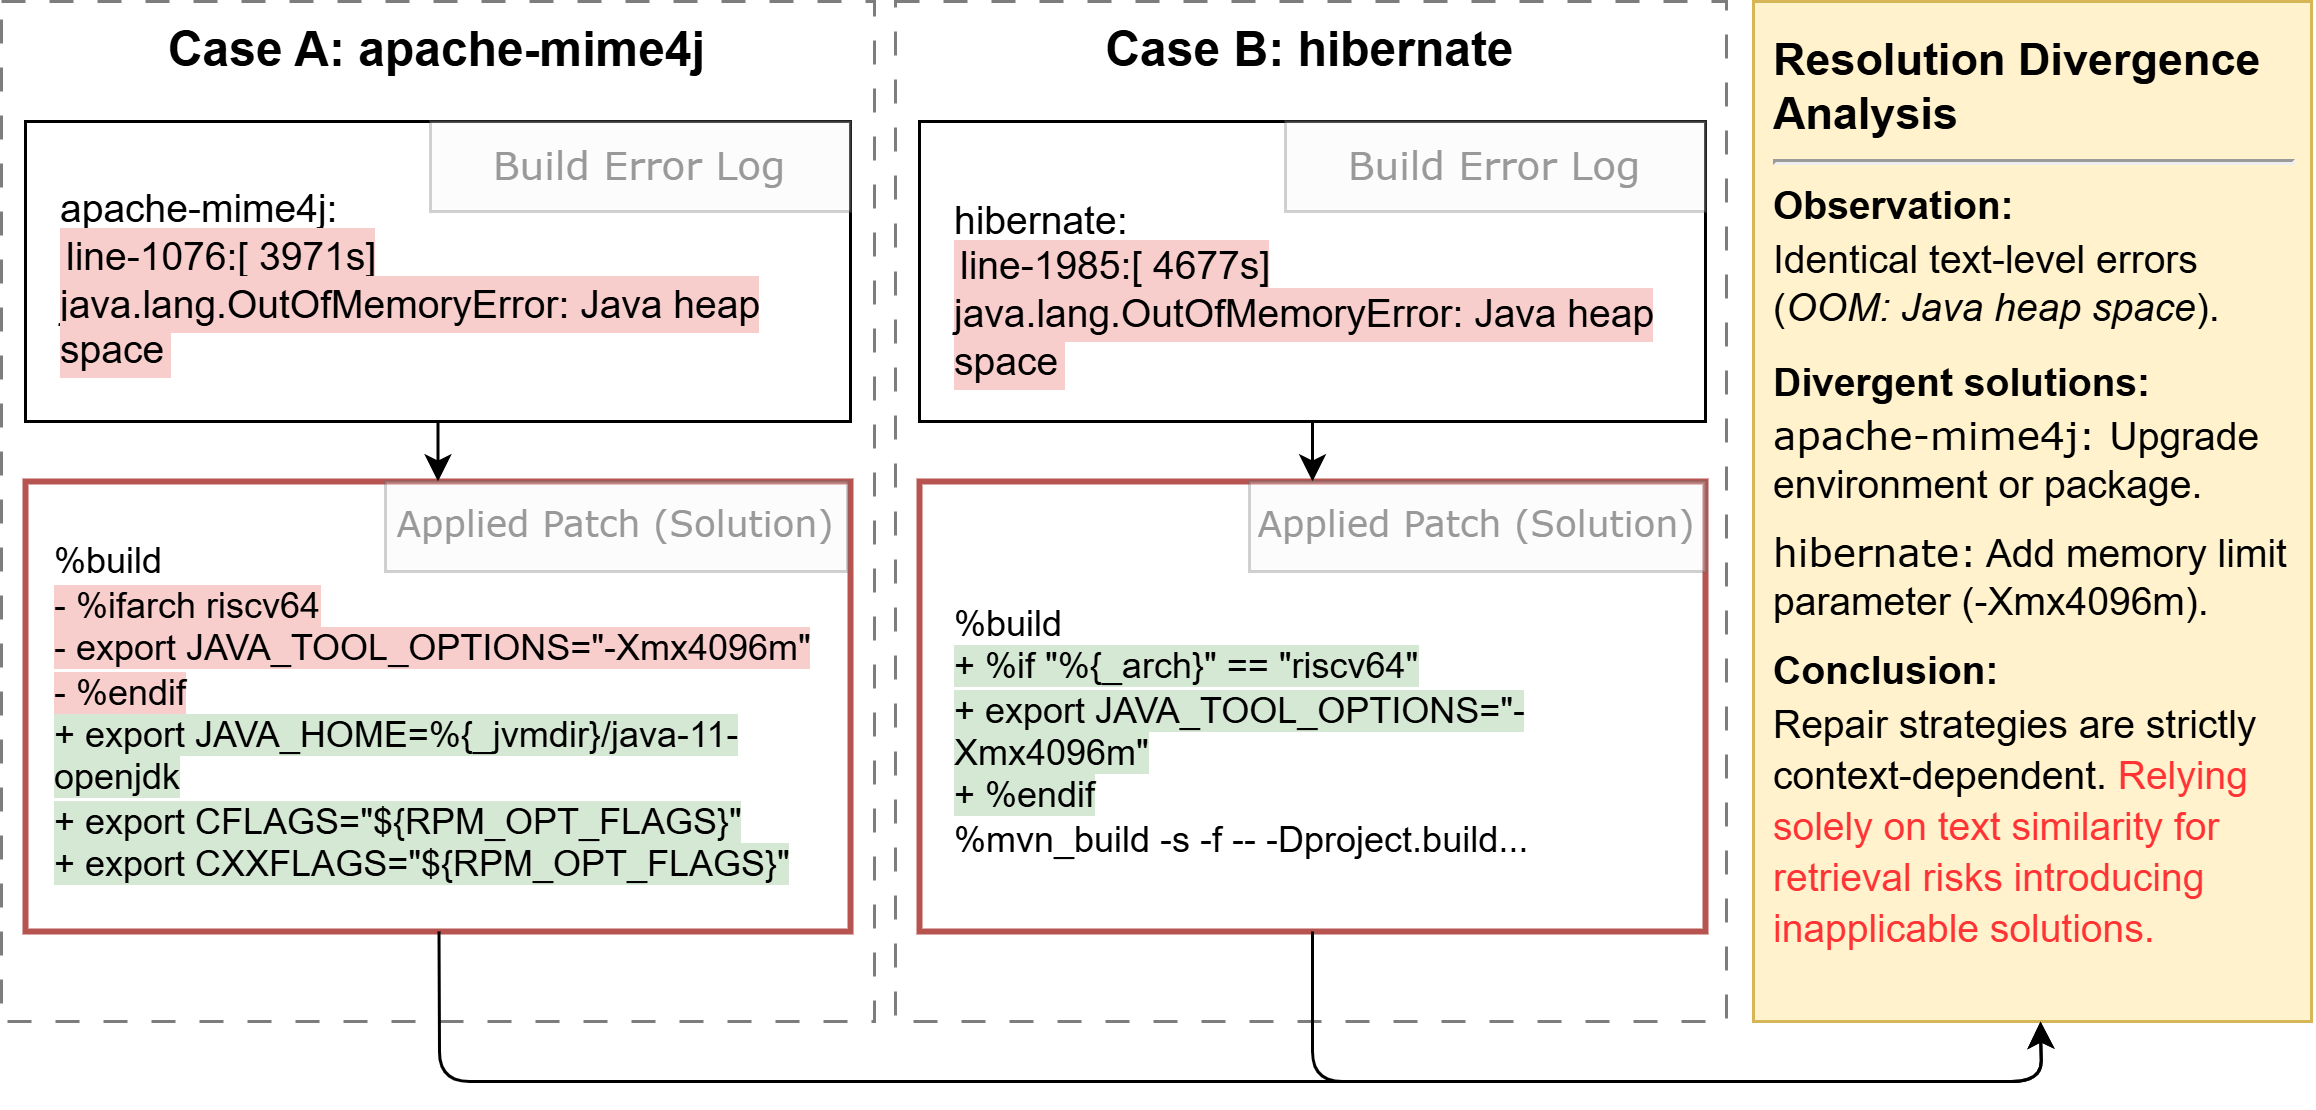
\includegraphics[width=\textwidth]{pic/similar-misleading.png}
        \caption{Similar errors but different fixes}
        \label{fig:similar-mislead}
    \end{subfigure}
    \caption{Motivating examples. (a) A build log with long-range causal dependency: the root cause at line 471 is far from the error at line 998. (b) Similarity misleading: two packages share the same error message but require different fixes.}
    \Description{Left: a build log snippet showing three highlighted regions illustrating long-range causal dependencies. Right: two build-log excerpts sharing the same error message but requiring different repair actions.}
\end{figure*}

In distribution-level package migration, platforms such as the Open Build Service (OBS) provide unified infrastructure for cross-distribution, cross-architecture package building through automated compilation, dependency resolution, and release management. Within such highly automated pipelines, however, build failures manifest with heightened frequency and diversity: the same package may fail on different architectures, under different dependency versions, or at different build stages (e.g., \texttt{\%prep}, \texttt{\%build}, \texttt{\%install}, \texttt{\%check}). These failures typically arise from a confluence of factors, including architectural incompatibilities, dependency-chain constraints, build-script misconfigurations, and patch inconsistencies. Build logs are voluminous---spanning tens of thousands to hundreds of thousands of lines---yet failure-relevant information constitutes fewer than 5\% of all lines, and log formats vary substantially across packages and stages. Moreover, the terminal error message frequently represents merely a downstream symptom; the underlying root cause may have manifested much earlier in the pipeline, giving rise to long-range causal dependencies.

To concretely illustrate these asynchronous triggering and long-range causal dependency patterns, Figure~\ref{fig:causal-dep} presents a representative build-log excerpt from the \texttt{aide} package. The failure exhibits a characteristic long-range distribution across the log: (1) \emph{Build termination signal (tail)}: the build system ultimately emits a generic termination signal (\texttt{RPM build errors}) at line 1021. (2) \emph{Explicit error statement (middle)}: tracing backward, the actual compilation error surfaces at line 998, where the log reports \texttt{`GCRY\_MD\_SM3' undeclared}. (3) \emph{Implicit root cause (head)}: the root cause of this undefined macro, however, resides in the dependency installation stage hundreds of lines earlier---at line 471, the system installs \texttt{libgcrypt-1.8.7-1.oe1}, a version lacking SM3 algorithm support. Notably, line 471 is an ostensibly benign \texttt{installing} entry bearing no anomaly markers.

This ``cause first, error later'' phenomenon underscores the fundamental challenge of analyzing ultra-long build logs: if automated analysis merely extracts a local window around the terminal error or filters lines by keywords such as \texttt{error}, the critical dependency-version evidence at line 471 is inevitably discarded. This motivates \textbf{Challenge 1}: how to locate the true root cause within an ultra-long log---key error lines are buried in voluminous noise, the actual root cause may have surfaced hundreds of lines earlier, and naive windowing around the terminal error readily misses upstream causal clues.

Even when the log compression stage successfully preserves the key evidence chain, root cause analysis and repair recommendation remain hampered by the absence of systematically organized historical knowledge. A naive vector-similarity-based RAG frequently encounters \emph{similarity misleading}: superficially similar logs do not necessarily warrant identical fixes. As illustrated in Figure~\ref{fig:similar-mislead}, the build logs of the \texttt{apache-mime4j} and \texttt{hibernate} packages share the same key error message, yet closer examination of their respective build scripts and environmental constraints reveals that the requisite fixes are fundamentally different. This example demonstrates that effective remediation depends not only on the error message itself but critically on contextual preconditions such as build stage, toolchain version, and dependency configuration. Relying solely on textual similarity for retrieval tends to surface cases whose applicability conditions are unmet, thereby elevating the risk of misdiagnosis.

Furthermore, the principal limitation of large language models in this domain lies not in their generative capacity but in the insufficient verifiability of their reasoning outputs. When multiple evidence fragments coexist, or when evidence is incomplete or mutually contradictory, models tend to produce fluent yet non-reproducible explanations. In engineering practice, diagnostic outputs must be auditable and reproducible, specifying not only the identified cause but also the supporting log evidence, the preconditions under which the diagnosis holds, and the corresponding historical repair records. This gives rise to \textbf{Challenge 2}: how to retrieve the \emph{right} historical fixes---repair knowledge is dispersed across commits and issue discussions spanning heterogeneous repositories; superficial log similarity does not guarantee fix applicability, as variations in version, dependency configuration, and build stage can render retrieved recommendations misleading.

For RISC-V package-migration build failures, there is accordingly a pressing need for an automated approach capable of preserving high-fidelity evidence chains within constrained token budgets while organizing historical repair knowledge into verifiable, condition-aware, and evidence-traceable representations.

Compared with the two-stage framework by Shuai et al.~\cite{shuai2025root}, which uses template-based log filtering and MCTS-guided free-form LLM generation, the present work advances the state of the art along two dimensions: (1) MGSC supersedes template matching with entity-driven long-range backtracking, achieving superior evidence coverage under more stringent token budgets; and (2) HRL-RCA replaces unconstrained LLM generation with structured rule-tree routing and evidence-bound reasoning, producing verifiable and interpretable repair recommendations rather than open-ended text.

To address the above challenges, this paper makes the following contributions:
\begin{enumerate}
\item We propose Multi-Granularity Semantic Compression (MGSC), a log compression method oriented to long-range causal dependencies. MGSC follows a three-stage pipeline of ``explicit error anchor localization---entity-based long-distance context backtracking---lightweight semantic compression'', and preserves high-fidelity evidence chains under strict token budgets.
\item We propose Historical Rule Learning for Root Cause Analysis (HRL-RCA). HRL-RCA structures historical repair experience into rules and organizes them into a tree index along the axes of ``error type---build stage---applicability conditions''. During online inference, it performs conditional routing to retrieve rules that satisfy their preconditions and, under a ReAct-style framework, generates traceable root cause analyses and repair suggestions.
\item Based on an OBS production environment, we construct a RISC-V build-failure dataset and conduct systematic experiments. Results show that MGSC achieves higher coverage of key evidence than existing compression methods, while HRL-RCA attains a comprehensive diagnostic score of 79.0\%, significantly outperforming various baselines, and reduces processing time by about 61\%.
\end{enumerate}

%% ===== Section 2 Related Work =====
\section{Related Work}

\subsection{Log Parsing and Semantic Compression}

Log parsing seeks to transform unstructured log data into structured representations comprising event templates and dynamic parameters. Early approaches relied on rules and regular expressions. Representative methods include SLCT~\cite{vaarandi2008mining}, which mines log patterns via clustering, Drain~\cite{he2017drain}, which constructs a fixed-depth parsing tree for efficient online parsing, and Logram~\cite{dai2020logram}, which employs $n$-gram dictionaries to accelerate template recognition. With the advent of deep learning, LSTM-based methods such as DeepLog~\cite{du2017deeplog} learn temporal patterns of normal execution paths for anomaly detection, while Transformer-based and self-supervised approaches yield stronger semantic representations~\cite{guo2021logbert,chen2022bert}. Semi-supervised methods such as PLELog~\cite{yang2021plelog} reduce annotation overhead, whereas LogGPT~\cite{qi2023loggpt} and LogLLM~\cite{guan2024logllm} directly leverage pre-trained language models for anomaly detection. Nevertheless, these methods often struggle to generalize across heterogeneous systems and evolving software versions~\cite{le2022log}.

More recently, large language models (LLMs) have introduced a new paradigm for log parsing~\cite{achiam2023gpt}. LogPrompt~\cite{liu2024logprompt}, a few-shot log-parsing method, reduces cost through judicious example selection; DivLog~\cite{xu2024divlog} enhances cross-domain parsing via in-context learning; LLMParser~\cite{ma2024llmparser} treats LLMs as generative parsers and provides systematic empirical analysis. LogShrink~\cite{li2024logshrink} specifically targets log compression by exploiting commonality and variability patterns. LogSage~\cite{xu2025logsage}, a log analysis framework for CI/CD scenarios, proposes token-efficient preprocessing and structured diagnosis. However, in build-failure scenarios involving software packages---where long-range causal dependencies and cross-stage reasoning are paramount---how to reliably preserve traceable evidence chains within stringent token budgets remains an open challenge necessitating task-specific compression strategies.

\subsection{Log-based Root Cause Analysis}

Root cause analysis (RCA) seeks to identify the underlying causes of failures from system outputs. Traditional approaches employ rule-based correlation to match events~\cite{notaro2023logrule}, or combine log analysis with source-code examination to infer failing execution paths~\cite{yuan2010sherlog}. Deep learning methods formulate RCA as a log-line relevance ranking problem, extracting indicative descriptions and parameters from logs for structured diagnosis~\cite{wittkopp2024logrca}. Knowledge-based approaches organize failure patterns into structured representations: LogKG~\cite{sui2023logkg} constructs knowledge graphs from log events for structured diagnosis, and Squeeze~\cite{li2019generic} performs multi-dimensional root cause localization.

LLM-based RCA emphasizes generating human-readable diagnostic conclusions directly from failure logs. Roy et al.~\cite{roy2024exploring} demonstrate that agent-based designs can mitigate the sensitivity of single-turn question answering to context budgets and incomplete information. RCAgent~\cite{wang2024rcagent} further validates the effectiveness of tool-augmented LLMs for cloud-based RCA, and PACE-LM~\cite{zhang2023pace} explores calibrated confidence estimation with GPT-4 for incident analysis. Shuai et al.~\cite{shuai2025root} propose a two-stage framework in which RV-LAD performs log compression and MCTS-RCA combines Monte Carlo tree search with RCA to guide LLM reasoning. However, approaches that rely solely on ``similar-log retrieval + free-form generation'' risk introducing misleading evidence and amplifying hallucinations; applicability conditions, evidence alignment, and verification mechanisms must be systematically incorporated. Our method explicitly distills verifiable rules from historical repair experience and organizes them into a rule tree with conditional routing, thereby mitigating the risk of misleading retrieval at its source.

\subsection{Build Failure Analysis and Package Migration}

Beyond general log analysis and RCA, a body of prior work specifically targets build failures. One line of research conducts empirical studies and pattern mining on build failures in large open-source ecosystems~\cite{rausch2017empirical}, aggregating failure records from distribution repositories and CI pipelines to characterize typical failure categories, error-prone stages, and their correlations with dependency relationships and configuration scripts, thereby establishing empirical foundations for automated repair. A complementary line of work, from a more engineering-oriented perspective, explores classification models and triage methods in CI build scenarios to automatically attribute and assign build failures~\cite{lee2024applying}, thereby reducing manual debugging effort.

However, these build-failure studies largely remain confined to a ``short window + local features'' paradigm: they either rely on manually crafted error patterns and heuristics that struggle with heterogeneous logs and cross-version evolution, or directly truncate lengthy logs into a single model input, thereby neglecting cross-stage long-range causal dependencies. Moreover, many existing systems focus on error-type prediction or simplistic heuristic recommendations and lack both structured organization of historical repair knowledge and explicit modeling of applicability conditions. In contrast, our work introduces MGSC to preserve evidence chains in long logs and HRL-RCA to model historical repair knowledge as a rule tree with explicit preconditions, achieving within a unified framework efficient long-log processing, cross-stage root cause localization, and verifiable repair recommendations.

\begin{figure*}[!tb]
    \centering
    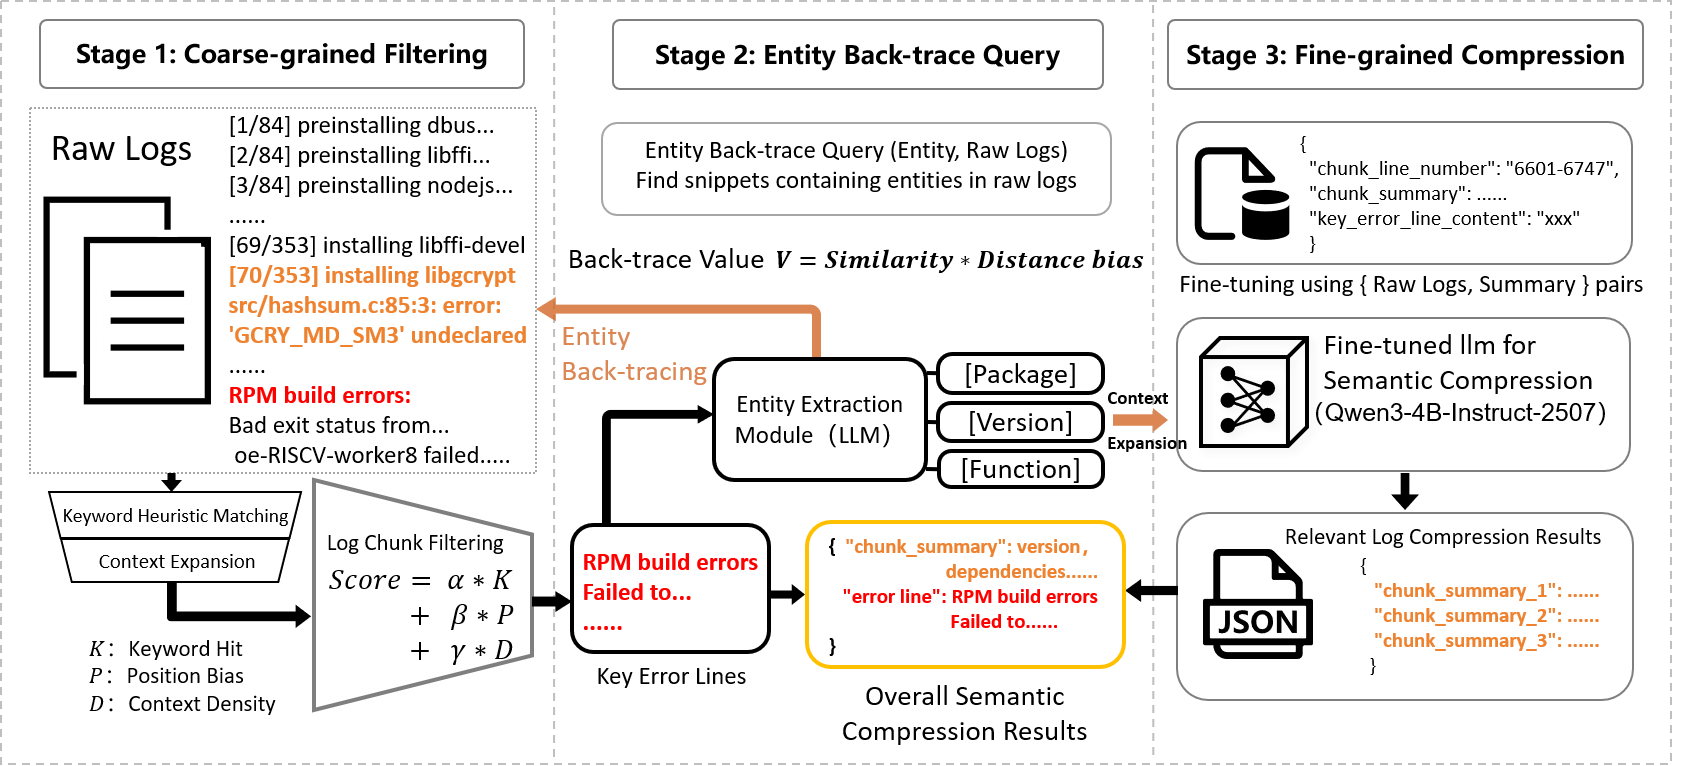
\includegraphics[width=\textwidth]{pic/mgsc-overview.png}
    \caption{Overall workflow of MGSC: Multi-Granularity Semantic Compression}
    \Description{A three-stage pipeline diagram: Stage 1 performs coarse-grained filtering with error anchor localization, Stage 2 performs entity-based context backtracking, and Stage 3 performs fine-grained semantic compression.}
    \label{fig:mgsc}
\end{figure*}

%% ===== Section 3 Method =====
\section{Method}

We adopt a two-stage pipeline for analyzing RISC-V build failures. In the first stage, MGSC performs multi-granularity semantic compression on ultra-long logs, producing a structured summary centered on key error lines with the necessary causal context. In the second stage, HRL-RCA consumes the compressed summary, combines it with a rule-tree index constructed from historical repair experience, and generates traceable root cause analyses and repair recommendations via conditional routing and ReAct-style reasoning.

\subsection{MGSC: Multi-Granularity Semantic Compression}\label{sec:mgsc}

Log compression for build-failure diagnosis is not merely a matter of discarding superfluous lines; the objective is to retain, within a constrained token budget, the critical evidence necessary for root cause analysis. To this end, we propose Multi-Granularity Semantic Compression (MGSC), a method specifically designed for long-range causal dependencies in build logs. The core idea is to first rapidly locate failure manifestations using explicit error information as anchors, then backtrack triggering conditions across long distances using key entities as clues, and finally perform fine-grained semantic compression and structuring over the candidate evidence set. In this manner, the original log is distilled into a summary that preserves causal information. MGSC emphasizes two design principles: multi-granularity and long-range association. Multi-granularity entails progressively focusing from key error lines, to error-related segments, and further to entity-level clues; long-range association is achieved through entity backtracking, which reconnects distant causal clues that would otherwise be lost under tail-only windowing. As shown in Figure~\ref{fig:mgsc}, MGSC consists of three stages: Stage 1 uses lightweight rules and heuristic scoring to prioritize segments near errors and critical turning points in the build process, obtaining candidate error blocks with high recall; Stage 2 extracts key entities from candidate blocks and backtracks them across the entire log to complete the causal chain; Stage 3 performs fine-grained semantic compression and structuring over the candidate segments, yielding a high-density information carrier under a fixed budget.

Given an original build log $L = \{l_1, l_2, \ldots, l_N\}$, the goal of MGSC is to produce a structured compressed result $S$ that satisfies a token-budget constraint $|S| \leq B$ while maximizing the coverage of key evidence and causal clues in $S$. Here $B$ is typically set to half of the downstream LLM's context window, leaving sufficient space for subsequent root cause reasoning and tool calls.

\subsubsection{Fast Coarse-Grained Filtering}

RISC-V package build logs on OBS are characteristically ultra-long, heterogeneous, and noisy. On one hand, logs contain voluminous routine compilation outputs, platform diagnostics, and toolchain metadata, while genuinely root-cause-relevant content constitutes only a minute fraction, yielding a very low signal-to-noise ratio. On the other hand, the build process spans multiple stages, and triggering conditions may first surface during early probing or dependency-checking stages yet manifest as explicit errors only later during compilation or linking. Applying entity backtracking or semantic compression directly to the full log is not only computationally prohibitive and token-intensive but also susceptible to interference from redundant information. Therefore, MGSC first performs a fast coarse-grained filtering stage, which quickly removes verified useless outputs using lightweight rules and heuristics, locates explicit error anchors, and generates a small set of highly relevant candidate blocks centered around those anchors.

Concretely, we first apply a set of regular-expression rules $R_{drop}$ to eliminate redundant outputs that recur across packages but bear no relevance to failures (e.g., compiler version echoes, download progress bars, fixed-format status messages), yielding a filtered log $L' = \{l_i \in L \mid g(l_i) = 1\}$. We then perform multi-level keyword matching to assemble a set of key error lines $A$, with matching tiers including: (1) strong error patterns such as \texttt{error:}, \texttt{fatal}, \texttt{undefined reference}, \texttt{No such file}, and \texttt{Bad exit status}; (2) build termination messages such as \texttt{RPM build errors} and \texttt{make: *** Error}; and (3) supplementary signals such as \texttt{undefined symbol} and \texttt{cannot find -lxxx}. Duplicate errors and repeated templates are merged to prevent a single error from consuming an excessive portion of the budget.

After obtaining the key error lines $A$, we expand a window around each error line to form candidate blocks $\mathcal{B}$, ensuring local semantic completeness. For each line $l_i$ in a block, we compute a line-level importance score:
\begin{equation}
S(l_i) = \alpha \cdot I_{key}(l_i) + \beta \cdot f_{pos}(i) + \gamma \cdot D_{context}(i)
\end{equation}
where $I_{key}$ is an indicator function for keyword matches, $f_{pos}(i) = e^{-\lambda(N-i)/N}$ is a positional bias term (lines closer to the log tail receive higher weights), and $D_{context}$ is a local keyword-density term. Block-level scores are obtained by aggregating line scores (e.g., max + mean), ensuring that blocks containing strong error anchors are ranked higher while avoiding an unfair advantage for longer blocks. The system ranks blocks by their scores and selects the Top-$n$ blocks under the token budget. In our setting, the total token length of this stage is constrained to be no more than one quarter of the downstream LLM's context window, leaving ample room for subsequent entity backtracking and semantic compression.

\subsubsection{Entity-Based Context Backtracking}

After coarse-grained filtering, the system has obtained a set of highly relevant candidate blocks anchored by explicit error lines that preserve the local context of failure manifestations. However, in RISC-V build-failure scenarios, relying solely on windowed snippets surrounding errors is frequently insufficient for reliable root cause analysis due to pronounced long-distance effects: the true triggering clues may appear earlier in \texttt{configure} checks, dependency installations, or configuration information, while final errors break out during \texttt{\%build}; the same root cause may manifest multiple times in different forms, for example, an early warning about missing headers/libraries, later compilation errors about undefined types/symbols, and final link-time \texttt{undefined reference} messages. This ``cause first, symptoms later'' long-range causal structure leads to broken evidence chains if we only preserve local windows around explicit errors.

To complete long-range causal chains, this stage extracts backtrackable query elements from explicit error segments and organizes them into a structured entity set $E$. Here, entities do not refer to arbitrary noun phrases in natural language but rather to symbolic clues that recurrently appear in build logs and point to key nodes in failure chains. These include function and symbol names (e.g., \texttt{\_\_cpuid}, \texttt{riscv\_v\_asm\_flag}), library names (e.g., \texttt{libatomic}, \texttt{openssl-devel}), missing headers, target files and paths, build targets, macros, and critical compiler or linker flags. The quality of $E$ directly governs backtracking effectiveness: an insufficiently populated entity set leads to inadequate recall, while an overly noisy set introduces irrelevant segments.

Using the entity set $E$ as queries, we search the original log $L$ for related segments. For each line $l_j$, we define a backtracking value:
\begin{equation}
V(l_j) = \max_{e \in E}\left(\mathrm{Sim}(l_j, e) \cdot \frac{1}{\log(1 + \lambda \Delta t(l_j, e))}\right)
\end{equation}
where $\mathrm{Sim}$ denotes fuzzy matching similarity (supporting substring matches, case-insensitive matches, and small edit distances), and the distance term biases toward closer lines when similarities are comparable. Lines whose values exceed a threshold are selected and aggregated into backtracking segments, thereby filling in causal evidence scattered across build stages. For example, when an explicit error reports \texttt{undefined reference to `foo\_v\_probe'}, entity backtracking may locate, in earlier \texttt{configure} stages, lines like \texttt{checking for foo\_v\_probe... no} and the corresponding compilation failures in \texttt{config.log}, thus bridging configuration-probing failures and link-time errors.

\subsubsection{Fine-Grained Semantic Compression}

After coarse-grained filtering and entity backtracking, the system has converged on two categories of valuable information: key error lines with their local context, and related segments recovered by backtracking entities across the entire log. However, these backtracking results still exist as raw log segments that may contain redundancy, exhibit stylistic inconsistency, and exceed acceptable length, risking overflow of the downstream model's context capacity. Naively concatenating them as LLM input would incur substantial token overhead and introduce noise and duplication that degrade the stability of subsequent reasoning.

Therefore, this stage performs fine-grained semantic compression. We use a lightweight, domain-tuned model to summarize and distill backtracking segments and then fuse them with explicit error information preserved in the coarse-grained stage, producing a structured and budget-controlled semantic summary of the log. Here, the summarization is task-oriented rather than generic: it focuses on information that supports RCA. On the one hand, it preserves context lines/segments helpful for localization; on the other, it attaches stage labels (e.g., \texttt{\%prep}, \texttt{\%build}) and distills key facts directly relevant to root causes, such as certain dependencies being disabled in \texttt{configure} due to missing packages, link-time failures like \texttt{cannot find -lxxx}, or architecture-specific symbols not being available under RISC-V.

We employ Qwen3-4B-Instruct as the base model, which exhibits strong instruction-following and text-generation capabilities at a moderate parameter scale suitable for cost-effective deployment. We apply supervised fine-tuning (SFT) with LoRA-based parameter-efficient tuning on 2,925 manually curated log-block compression examples to guide the model toward preserving critical information, compressing uninformative content, and producing stable output formats. Experiments demonstrate that the compression ratio improves from 19.66$\times$ to 30.6$\times$, while key-error coverage increases marginally from 74.3\% to 75.7\%, confirming that domain-specific tuning enhances compression efficiency without sacrificing essential information.

Finally, we fuse the fine-grained summaries with explicit error information from the coarse-grained stage to obtain the structured compressed result $S$, which is human-readable, reproducible, and well-suited for subsequent rule-based root cause reasoning.

\begin{figure*}[!t]
    \centering
    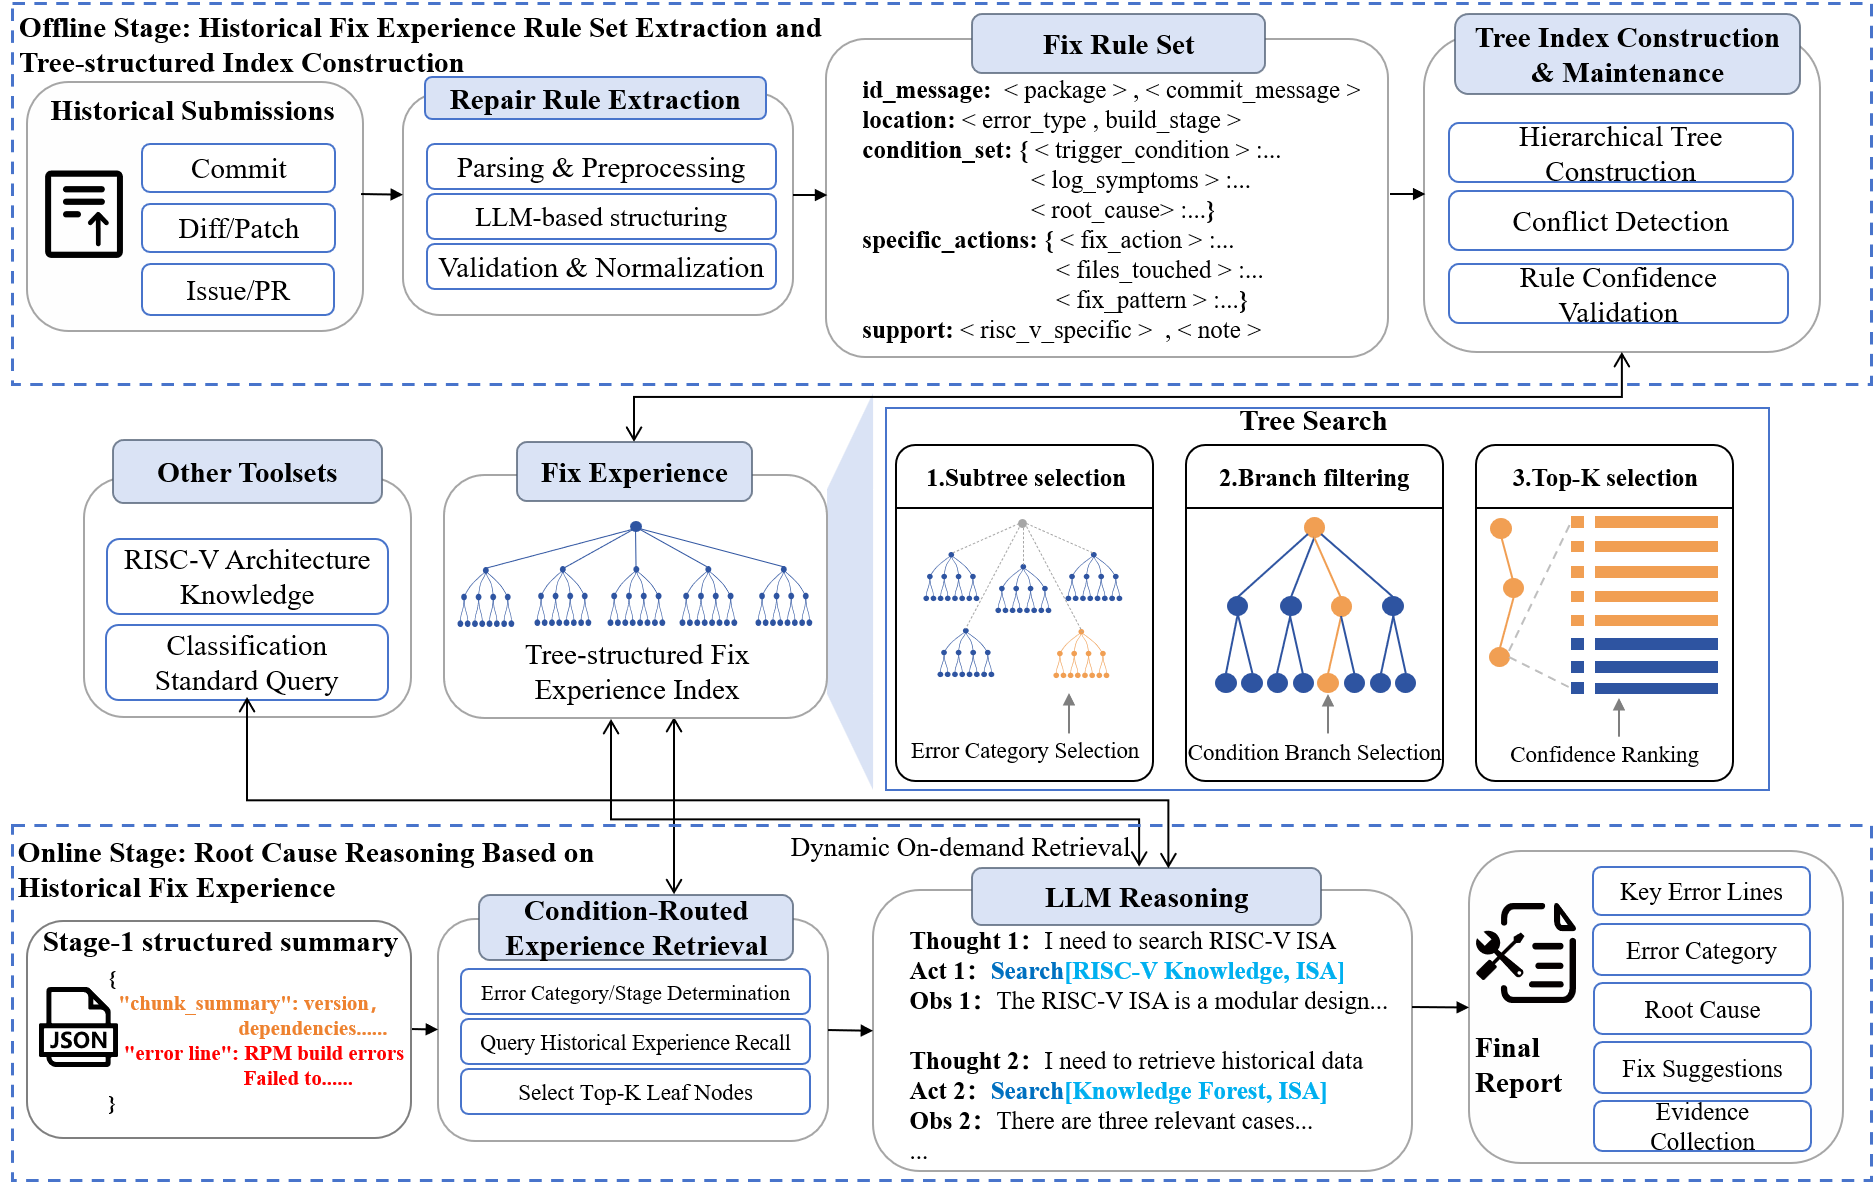
\includegraphics[width=\textwidth]{pic/hrl-rca-overview.png}
    \caption{HRL-RCA: framework of Historical Rule Learning for Root Cause Analysis}
    \Description{A framework diagram showing offline rule extraction from historical commits and online conditional routing over a rule tree for root cause analysis.}
    \label{fig:hrl-overview}
\end{figure*}

\subsection{HRL-RCA: Historical Rule Learning for Root Cause Analysis}\label{sec:hrl}

To mitigate the similarity misleading inherent in naive similarity-based retrieval and to ensure that repair recommendations are verifiable with explicit evidence, we propose Historical Rule Learning for Root Cause Analysis (HRL-RCA). The fundamental idea is to extract and explicitly structure the relationships among ``symptoms---applicability conditions---repair actions---evidence'' from historical repair records, transforming scattered experience into reusable repair rules, and to construct a maintainable rule-tree index along axes of problem category, build stage, and verifiable conditions. During online inference, rather than retrieving by similarity directly, we use the MGSC summary as input for conditional routing over the rule tree, activating rules only when their applicability conditions are satisfied, and subsequently generating root cause explanations and fixes under explicit evidence constraints. This paradigm yields interpretable, traceable, and actionable diagnostic outputs.

As shown in Figure~\ref{fig:hrl-overview}, the overall workflow contains an offline construction and an online inference part. Offline, we process historical repair commits to extract and structure repair experience from commit messages, diffs/patches, and packaging-related spec changes, and store them as reusable rules. Then, we construct a rule-tree skeleton organized by error category and build stage, and attach each rule to leaf nodes whose conditions are satisfied, with conflict detection and incremental updates. Online, we take the MGSC summary $S$ (optionally augmented with spec/patch and environment summaries) as input, first determine error type and build stage to locate the entry in the rule tree, and then traverse conditional branches to retrieve candidate leaf rules. Under evidence constraints, we finally generate a diagnostic report containing ``root cause---fix---applicability conditions---evidence references''.

\subsubsection{Structuring Historical Repair Information}

In practice, historical repair experience is primarily recorded in version-control commits, encompassing commit messages, code diffs/patches, and packaging-related spec changes. Although these artifacts contain rich repair knowledge, they are inherently unstructured, stylistically heterogeneous, and varied in evidence granularity: the same category of problem may be described in disparate terms (e.g., ``fix build'', ``riscv workaround'', ``linker error''), while the actual executable repair actions are often embedded within diff fragments. Directly using raw commits as retrieval targets in similarity-based methods readily reintroduces similarity misleading and fails to explicitly capture the relationship between applicability conditions and repair actions. Therefore, HRL-RCA first abstracts historical commits into structured units---repair rules---thus elevating experience from free text to computable, routable, and maintainable knowledge items.

\begin{sloppypar}
Rule construction takes a single repair commit as the basic object, with inputs including: (1) commit message describing intent and background; (2) diffs/patches containing concrete code or script changes; (3) spec changes related to packaging (e.g., dependency declarations, macro and build-parameter modifications, patch references); and (4) associated issue/PR discussions providing information about reproduction, applicability conditions, and boundary cases. The output is a structured JSON record whose fields emphasize two aspects. First, applicability conditions are explicitly encoded (e.g., \texttt{error\_type}, \texttt{build\_\-stage}, \texttt{trigger\_\-condition}, \texttt{risc\_v\_\-specific}, \texttt{can\_\-generalize}) to support later tree construction and conditional routing. Second, evidence carriers (e.g., \texttt{files\_\-touched}, \texttt{commit\_id}, \texttt{notes}) are preserved to ensure traceability and human verification.
\end{sloppypar}

\begin{sloppypar}
The construction pipeline adopts a three-stage process: ``traditional parsing and preprocessing---LLM-based structuring---validation and normalization''. First, we use traditional techniques to pre-parse metadata and changes, including segmenting commit messages, diffs/patches, spec changes, and associated issue/PR content, and extracting salient elements such as touched files, key change hunks, dependency declarations, and macro/parameter modifications. This reduces input noise and provides structural hints for LLMs. Second, with unified prompt templates and fixed output schemas, we invoke an LLM to convert parsed results into structured repair rules, covering fields such as \texttt{error\_type}, \texttt{build\_\-stage}, \texttt{trigger\_\-condition}, \texttt{root\_\-cause}, and \texttt{fix\_\-action}, and mapping key fields such as triggers and fix patterns to predefined label sets whenever possible. Finally, an independent validation module automatically checks LLM outputs: it verifies schema conformance (field completeness, type consistency, non-empty required fields) and performs normalization consistency checks for \texttt{fix\_\-action} and \texttt{trigger\_\-condition}. When validation fails, the system triggers a rewrite strategy, asking the model to regenerate specific fields using feedback from validation, ensuring that only rules with stable formats, routable conditions, and traceable evidence enter the knowledge base.
\end{sloppypar}

\subsubsection{Rule-Tree Index Construction and Maintenance}

After obtaining structured rules, we must organize the dispersed repair experience into a routable and maintainable knowledge structure. We adopt a tree index for knowledge organization for three reasons. First, the manual diagnostic workflow for build failures inherently follows a decision path of first determining error category and build stage, then narrowing down by applicability conditions. A tree index explicitly encodes this process as conditional branches, rendering rule-matching paths naturally interpretable and auditable. Second, the effectiveness of repair experience is strongly conditioned on prerequisites (e.g., software versions, target architecture, dependency states, build systems, and build stages). Tree routing mandates that each step satisfy verifiable conditions, filtering out inapplicable rules at the retrieval entry point and thereby mitigating the risks of erroneous retrieval due to superficial similarity. Third, supplying all rules and their conditions to an LLM for ad-hoc conditional retrieval would entail prohibitive token costs, and the model would be susceptible to attention dispersion and overlooked conditions amid the resulting redundancy. The tree index pre-materializes the routing structure, performing structural pruning prior to LLM inference and injecting only the small subset of rules that satisfy the current conditions, thus enabling compact-context, strongly constrained, and auditable reasoning.

As illustrated in Figure~\ref{fig:rule-tree}, we start from a root node and split the first layer into five domains in accordance with our error taxonomy (architecture compatibility, version compatibility, dependency configuration, build configuration, and other errors), so that online inference can first perform coarse routing at the problem-domain level. The second layer is organized by build stage (e.g., \texttt{\%prep}, \texttt{\%build}, \texttt{\%install}, \texttt{\%check}), constraining historical experience to consistent stage contexts to avoid misinterpretation of the same error text under different stages. Deeper nodes branch according to verifiable routing conditions derived from \texttt{trigger\_condition} and \texttt{log\_symptoms} in rules, such as ``whether dependency xxx is detected missing'', ``whether the failure only occurs on RISC-V'', etc. Leaf nodes store sets of concrete repair rules with their \texttt{fix\_action}, applicability conditions, and annotations. Once a path is hit during online inference, the system obtains a joint package of ``conditions---actions---evidence''.

\begin{figure}[!htbp]
    \centering
    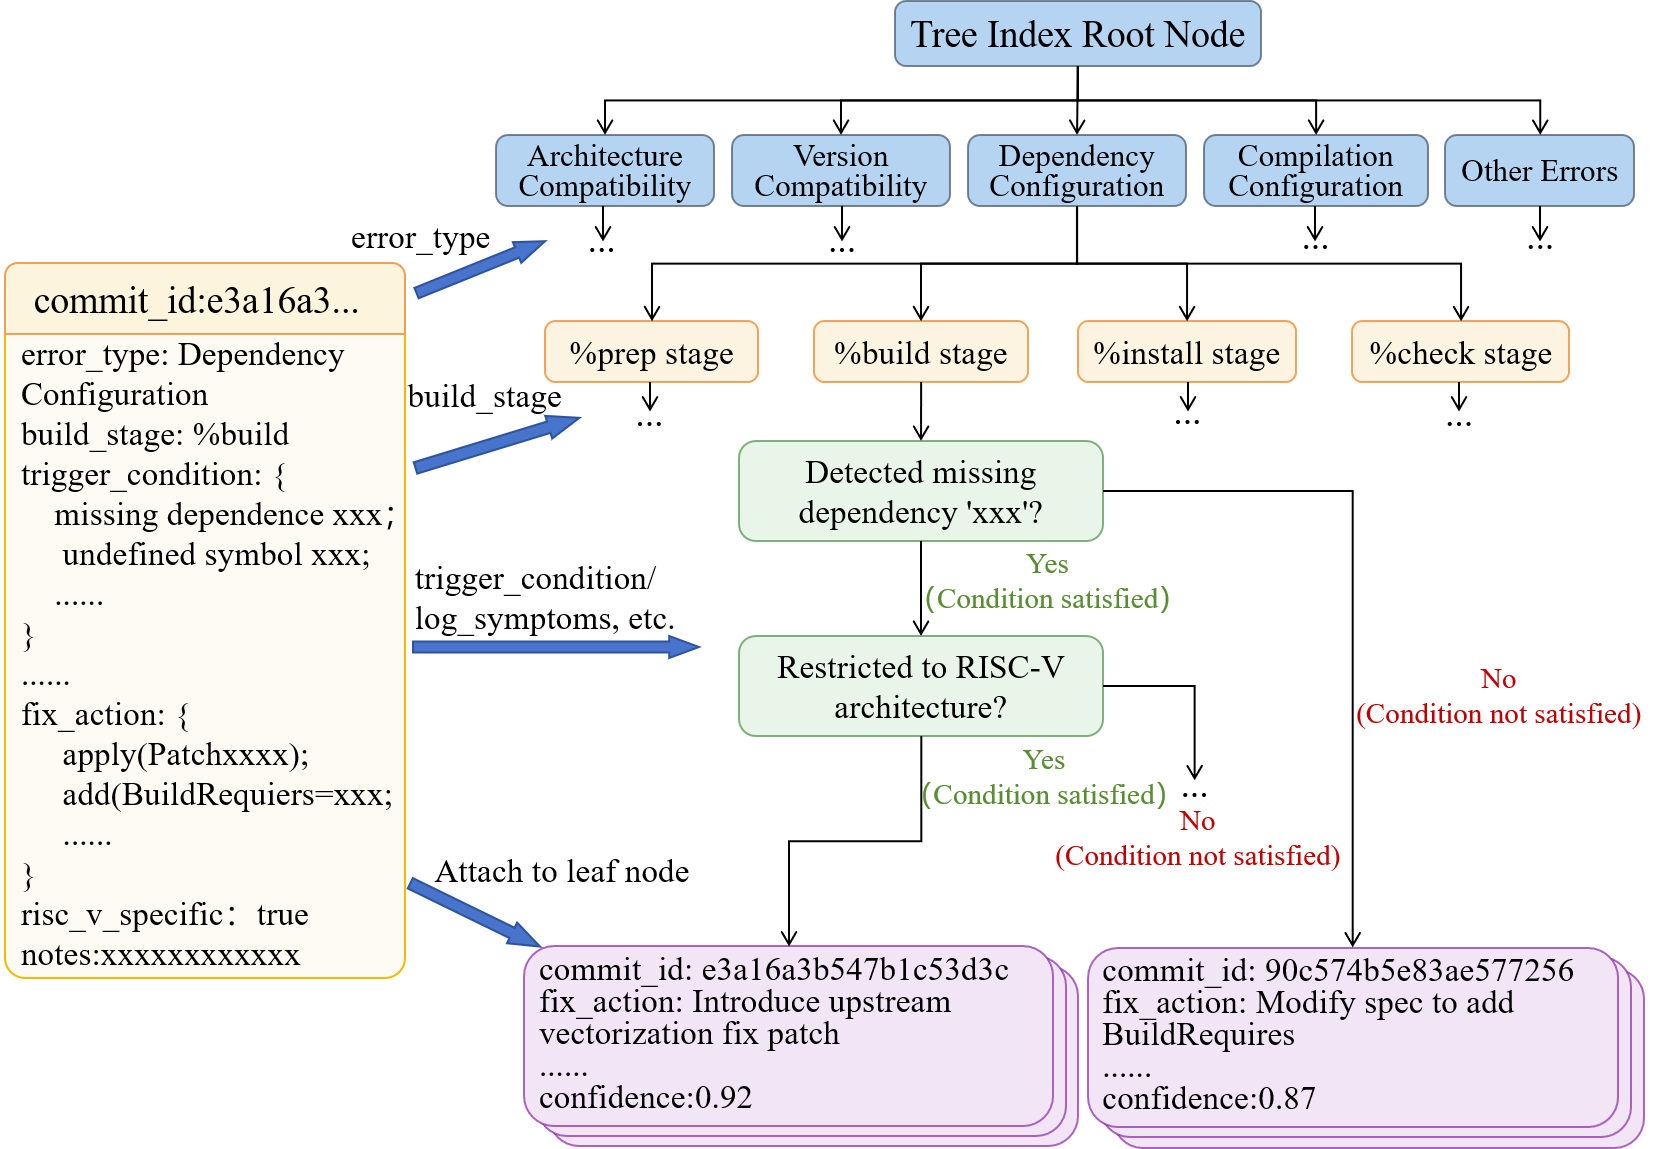
\includegraphics[width=\columnwidth]{pic/rule-tree.png}
    \caption{Illustration of the rule-tree index structure}
    \Description{A tree diagram with the root branching into five error categories, each further split by build stage, and leaf nodes storing structured repair rules.}
    \label{fig:rule-tree}
\end{figure}

To support continuous evolution, we design incremental updates and conflict-resolution mechanisms. Given a new rule, we first normalize it using the same offline procedure and then determine its routing position. If the condition set $C_{new}$ of the new rule and $C_{old}$ of an existing rule have inclusion relationships, we handle them as follows: when $C_{new} \supset C_{old}$, the new rule has stricter conditions, so we add a deeper branch in the tree and give the fine-grained rule higher priority; when $C_{new} \subset C_{old}$, the new rule is more general, and we adjust the tree to generalize conditions and reduce duplicate branches. This avoids naive stacking of rules that would lead to path explosion.

We further introduce rule confidence for quality control:
\begin{equation}
\mathrm{Conf}(r) = \alpha \cdot S_{evi}(r) + (1-\alpha) \cdot S_{time}(r)
\end{equation}
where $S_{evi}(r) = n_r / (n_r + k)$ is evidence support (with $n_r$ being the number of supporting records and $k$ a smoothing constant, default $k{=}3$), and $S_{time}(r) = 1 / (1 + (t_{now} - t_r)/T)$ measures recency (with $T{=}90$ days, meaning the recency drops to 0.5 after 90 days). Rules whose confidence falls below a threshold are used only as low-priority candidates and placed in a queue for manual review; only those above the threshold become high-priority leaf evidence for routing. This mechanism jointly constrains knowledge quality and freshness during incremental evolution.

\subsubsection{Online Root Cause Reasoning}

In the online phase, given a build-failure instance, the objective is to perform conditional routing and historical-experience retrieval along the rule tree, and then, under explicit evidence constraints, generate interpretable, actionable, and verifiable root cause analyses and repair recommendations. We adopt a ReAct-style evidence-driven reasoning framework, employing the MGSC summary $S$ as the entry point and encapsulating external knowledge queries and rule-tree retrieval as invocable tools. The model then iterates between ``acting'' and ``observing'' to progressively accumulate evidence and converge on applicable rules.

\textbf{Error type and stage determination.} The first step is to determine the error category and build stage of the current failure. The MGSC summary $S$ already encodes explicit error lines, stage-related clues, key entities, and supporting evidence snippets. If $S$ explicitly contains stage information, we use it directly; otherwise, we infer the stage from characteristic patterns surrounding the error anchors. For error categorization, we map error anchors and entities in $S$ to one of our five predefined categories via a standardized decision procedure. When $S$ reveals architecture-specific entities or patterns, we optionally invoke RISC-V knowledge tools for supplementary verification to prevent misclassification based solely on surface-level error messages.

\textbf{Retrieving relevant historical repair experience.} After determining error type and stage, we query the rule tree. We first locate the appropriate problem-domain node according to \texttt{error\_type} and then descend into the corresponding stage subtree according to \texttt{build\_stage}, confining candidates to a semantically coherent region. Within the stage subtree, we use triggers and key entities extracted from $S$ to evaluate branch conditions. We traverse top-down: when evidence unambiguously satisfies a branch condition, we follow it; when evidence is insufficient for a definitive judgment, we retain the branch as a candidate to avoid premature pruning; when evidence explicitly contradicts a branch, we skip it. If multiple leaf nodes remain, we rank their rules by matching degree (coverage of triggers and entities) and rule confidence, retaining the Top-$K$ rules as candidate evidence. If no leaves are matched, we back off to higher-level nodes and fall back to more general rules.

\textbf{ReAct-style reasoning.} Upon retrieving candidate rules, we proceed to diagnostic output generation. Three categories of information are assembled in the LLM context: (1) the MGSC summary $S$, providing error anchors, stage clues, and entities; (2) retrieved historical rules (Top-$K$ candidates); and (3) routing path metadata (problem domain, stage, and branch sequence). Following the ReAct paradigm, the model first formulates preliminary hypotheses based on $S$ and the candidate rules. If it identifies missing critical information or inconsistencies among candidates, it issues ``actions'' to invoke tools (e.g., RISC-V knowledge queries or validation of hypothetical fixes), incorporates tool outputs as ``observations,'' and then refines its hypotheses accordingly. The model is required to produce a structured diagnostic report comprising: (1) key error and stage localization; (2) error-type classification with rationale; (3) a verifiable root cause explanation; (4) concrete, executable repair recommendations; and (5) supporting evidence with references to historical repairs. When multiple candidate rules remain plausible, the system outputs a primary recommendation alongside alternatives, each annotated with its \texttt{trigger\_condition} delineating applicability boundaries, thereby avoiding unverifiable compromises when evidence conflicts.

%% ===== Section 4 Evaluation =====
\section{Evaluation}

We evaluate our approach by addressing four research questions:
\begin{itemize}[leftmargin=*]
\item \textbf{RQ1 (Log Compression):} How effective is MGSC in preserving key evidence compared with existing log compression methods?
\item \textbf{RQ2 (Ablation):} What is the contribution of each MGSC component?
\item \textbf{RQ3 (Root Cause Analysis):} How does HRL-RCA compare with baselines in diagnostic quality?
\item \textbf{RQ4 (Efficiency):} How efficient is HRL-RCA in terms of processing time?
\end{itemize}

\subsection{Experimental Setup}

\subsubsection{Datasets}
\begin{sloppypar}
Our experimental data are drawn from RISC-V package build-failure logs in a production OBS environment. For log compression, we use build logs from 133 distinct packages, totaling 149{,}219 log lines. Domain experts annotated 4{,}582 key repair-related lines as ground truth. For root cause analysis, we use 174 representative build-failure cases spanning five error categories (architecture compatibility, build configuration, dependency configuration, version compatibility, and other errors). This dataset extends the 117-case corpus used by Shuai et al.~\cite{shuai2025root} with additional cases encompassing more diverse packages and failure patterns.

As shown in Figure~\ref{fig:dataset}, version-compatibility errors account for the largest proportion (29.9\%), while build-configuration and dependency-configuration errors each account for 23.6\%, other errors 14.4\%, and architecture-compatibility errors 8.6\%. Regarding build-stage distribution, 50.0\% of failures occur in \texttt{\%build}, 24.1\% in \texttt{\%prep}, 20.7\% in \texttt{\%check}, and 5.2\% in \texttt{\%install}.
\end{sloppypar}

\begin{figure}[!htbp]
    \centering
    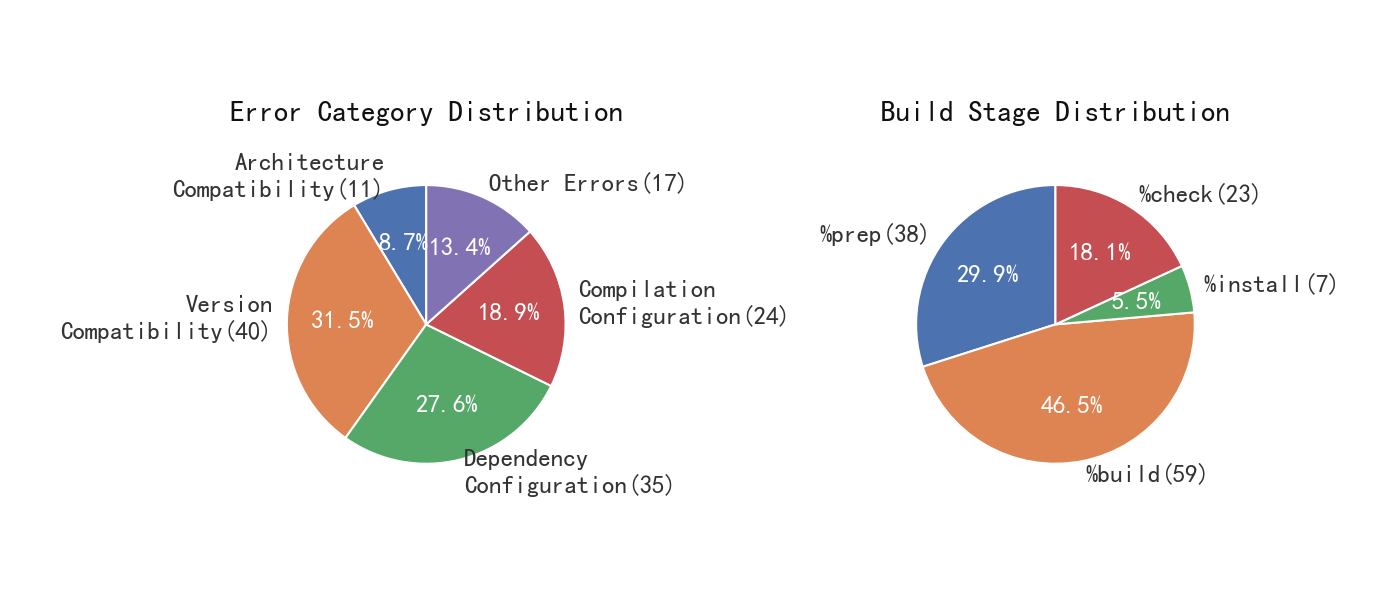
\includegraphics[width=\columnwidth]{pic/dataset-dist.png}
    \caption{Distribution of error categories and build stages in the RISC-V build-failure dataset}
    \Description{Two pie charts showing the distribution of five error categories and four build stages in the dataset.}
    \label{fig:dataset}
\end{figure}

\subsubsection{Baselines}
For log compression, we compare MGSC with three baselines: (1) LogSage~\cite{xu2025logsage}, an LLM-based analysis framework for long logs; (2) TemplateRAG~\cite{shuai2025root}, a template-based parsing and retrieval-augmented method; and (3) LogPrompt~\cite{liu2024logprompt}, which enhances LLM-based log analysis via prompt engineering.

For root cause analysis, we consider four classes of baselines: (1) a naive RAG agent based on semantic-similarity retrieval and generation; (2) LogSage~\cite{xu2025logsage}, which uses improved multi-path RAG retrieval; (3) MCTS~\cite{shuai2025root}, a search-based reasoning framework; and (4) flagship reasoning models (Seed~1.8\footnote{Seed 1.8: a reasoning model developed by ByteDance.}, Kimi~K2\footnote{Kimi K2: a reasoning model developed by Moonshot AI.}, DeepSeek-V3.2), which primarily rely on model capacity improvements.

\subsubsection{Implementation Details}
For HRL-RCA and all baselines, we use DeepSeekV3 and GPT-OSS as backbone LLMs. Standalone reasoning models are evaluated end-to-end with MGSC-compressed log summaries as input. The MGSC fine-tuned compression model uses Qwen3-4B-Instruct with LoRA-based parameter-efficient tuning (details in Section~\ref{sec:mgsc}). The rule-tree knowledge base is constructed offline from historical OBS repair commits following the procedure described in Section~\ref{sec:hrl}.

\subsubsection{Metrics}
\begin{sloppypar}
For log compression, we use line-level Precision/Recall/F1 to evaluate the preservation of key evidence. For root cause analysis, we adopt a composite score:
\begin{equation}
\text{score}(i) = \frac{s_i + c_i + r_i + f_i}{4}
\end{equation}
where $s_i$ is the score for extracting key error statements, $c_i$ for error classification, $r_i$ for root cause explanation, and $f_i$ for repair suggestion. Each sub-score ranges from 0 to 1 and is assessed by three domain experts following a rubric: 1.0 (fully correct), 0.75 (mostly correct with minor omission), 0.5 (partially correct), 0.25 (mentioned but largely incorrect), and 0 (missing or wrong). The final score for each sub-dimension is the majority vote among the three annotators. Inter-annotator agreement measured by Fleiss' $\kappa$ is 0.72, indicating substantial agreement.
\end{sloppypar}

\subsection{RQ1: Effectiveness of MGSC for Log Compression}

\begin{table}[htbp]
\centering
\caption{Accuracy comparison of log compression methods}
\label{tab:mgsc-results}
\begin{tabular}{lccc}
\hline
\textbf{Method} & \textbf{Prec} & \textbf{Rec} & \textbf{F1} \\
\hline
LogPrompt & 0.260 & 0.300 & 0.334 \\
TemplateRAG & 0.047 & \textbf{0.769} & 0.080 \\
LogSage & \textbf{0.308} & 0.574 & 0.387 \\
MGSC (ours) & 0.302 & 0.668 & \textbf{0.389} \\
\hline
\end{tabular}
\end{table}

As shown in Table~\ref{tab:mgsc-results}, MGSC achieves a Recall of 0.668, substantially surpassing LogSage (0.574), indicating that the combination of error-anchor-based coarse filtering and entity backtracking more effectively recovers key clues along long-range causal chains. Simultaneously, MGSC attains considerably higher Precision than TemplateRAG (0.302 vs.\ 0.047), demonstrating that MGSC can suppress large volumes of irrelevant noise while improving coverage. In terms of token efficiency, MGSC's average output lengths for three groups of logs are 3442/4234/5502 tokens, consistently in the low-thousands range and one order of magnitude smaller than TemplateRAG (38746/49883/55406), reserving ample context budget for subsequent reasoning. Regarding runtime, MGSC achieves approximately 2.3--3.6$\times$ speedup over LogPrompt and TemplateRAG on ultra-long logs.

\subsection{RQ2: Contribution of Each MGSC Component}

We perform an ablation study to assess the contribution of each MGSC component.

\begin{table}[htbp]
\centering
\caption{Ablation results of MGSC}
\label{tab:mgsc-ablation}
\begin{tabular}{lccc}
\hline
\textbf{Configuration} & \textbf{Prec} & \textbf{Rec} & \textbf{F1} \\
\hline
MGSC (full) & 0.302 & 0.668 & 0.389 \\
w/o Anchor Filter & 0.274 & 0.352 & 0.328 \\
w/o Entity Backtracking & 0.292 & 0.584 & 0.372 \\
w/o Semantic Compressor & 0.246 & 0.668 & 0.349 \\
\hline
\end{tabular}
\end{table}

As shown in Table~\ref{tab:mgsc-ablation}, removing error-anchor-based coarse filtering (w/o Anchor Filter) reduces Recall from 0.668 to 0.352 (a 47.3\% decrease) and lowers F1 by 15.7\%, demonstrating that explicit anchor localization is essential for rapidly focusing on anomalous regions. Removing entity backtracking (w/o Entity Backtracking) decreases Recall and F1 by 12.6\% and 4.4\%, respectively, confirming that this module effectively recovers long-distance causal clues. Without the semantic compressor (w/o Semantic Compressor), Recall remains unchanged but Precision declines by 18.5\%, indicating that the lightweight compressor primarily enhances output purity and structural consistency of the generated summaries.

\subsection{RQ3: Comparison with Baselines on Root Cause Analysis}

\begin{table}[htbp]
\centering
\caption{Overall performance comparison on root cause analysis}
\label{tab:hrl-results}
\small
\setlength{\tabcolsep}{3pt}
\begin{tabular}{llccccc}
\hline
\textbf{Group} & \textbf{Method} & $s_i$ & $c_i$ & $r_i$ & $f_i$ & \textbf{Score} \\
\hline
\multirow{4}{*}{{\footnotesize DeepSeekV3}}
& RAG & 0.769 & 0.657 & 0.655 & 0.520 & 0.650 \\
& LogSage & 0.870 & 0.754 & 0.692 & 0.524 & 0.710 \\
& MCTS & 0.881 & 0.777 & 0.714 & 0.567 & 0.735 \\
& HRL-RCA & \textbf{0.892} & \textbf{0.798} & \textbf{0.766} & \textbf{0.706} & \textbf{0.790} \\
\hline
\multirow{4}{*}{{\footnotesize GPT-OSS}}
& RAG & 0.743 & 0.625 & 0.693 & 0.613 & 0.669 \\
& LogSage & 0.791 & 0.699 & 0.721 & 0.606 & 0.704 \\
& MCTS & \textbf{0.841} & \textbf{0.747} & 0.754 & 0.590 & 0.733 \\
& HRL-RCA & 0.821 & 0.745 & \textbf{0.760} & \textbf{0.742} & \textbf{0.767} \\
\hline
\multirow{3}{*}{{\footnotesize \shortstack{Reasoning\\Models}}}
& Seed 1.8 & 0.814 & 0.665 & 0.755 & 0.635 & 0.717 \\
& Kimi K2 & 0.833 & 0.713 & 0.744 & 0.592 & 0.721 \\
& DSV3.2 & 0.728 & 0.605 & 0.691 & 0.545 & 0.642 \\
\hline
\end{tabular}
\end{table}

As shown in Table~\ref{tab:hrl-results}, HRL-RCA consistently achieves the highest comprehensive scores across both backbone configurations. With DeepSeekV3 as the backbone, HRL-RCA attains an overall score of 0.790, outperforming the strongest baseline MCTS (0.735) by 5.5 percentage points and the naive RAG agent (0.650) by 21.5\%.

\begin{figure}[!htbp]
    \centering
    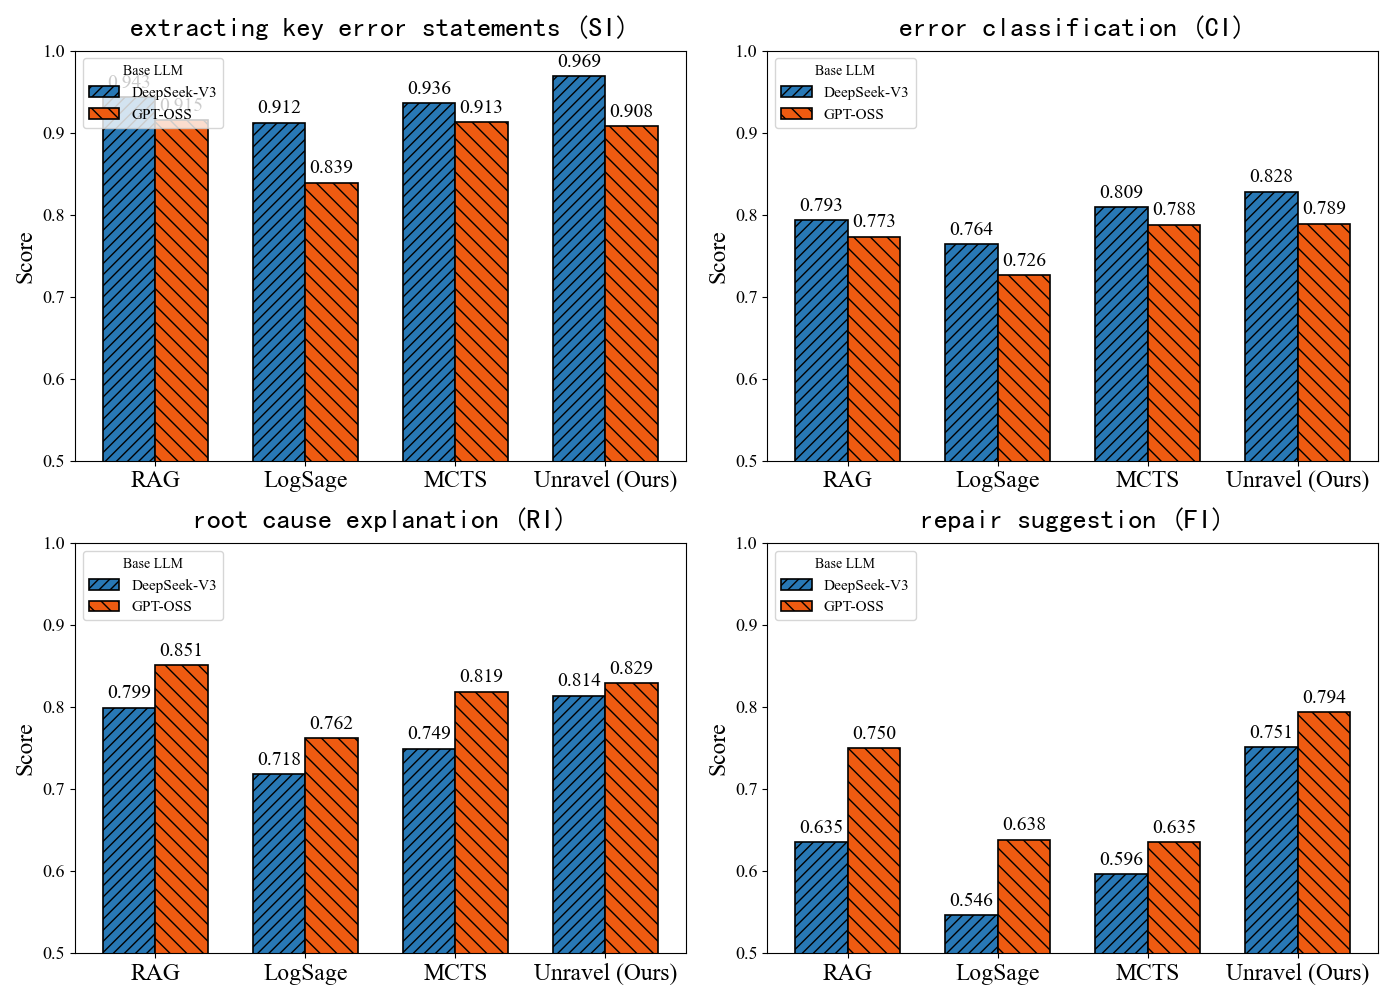
\includegraphics[width=\columnwidth]{pic/HRL-RCA-exp.png}
    \caption{Per-metric score comparison across methods}
    \Description{A grouped bar chart comparing key-error extraction, classification, root cause, and repair scores across RAG, LogSage, MCTS, and HRL-RCA methods.}
    \label{fig:sub-scores}
\end{figure}

Figure~\ref{fig:sub-scores} reveals that HRL-RCA's primary advantages reside in repair recommendation and root cause explanation. With DeepSeekV3, HRL-RCA achieves a repair-suggestion score of 0.706, exceeding MCTS (0.567) by 0.139. This indicates that conditional routing and evidence binding grounded in historical repair rules facilitate the recall of executable fixes whose preconditions are satisfied. Scores for key-error extraction are relatively high across all methods (0.769--0.892), suggesting that the upstream log compression already provides robust error anchors; HRL-RCA nonetheless achieves the highest score (0.892), reflecting the stabilizing effect of structured reasoning pathways.

Compared with standalone flagship reasoning models, Seed~1.8, Kimi~K2, and DeepSeek-V3.2 all yield lower scores than HRL-RCA. This finding suggests that for build-failure diagnosis---where applicability conditions and verifiable evidence are paramount---merely scaling model capacity is insufficient to ensure high-quality repair recommendations; structured knowledge organization and evidence constraints are indispensable.

\subsection{RQ4: Efficiency Analysis}

\begin{figure}[!htbp]
    \centering
    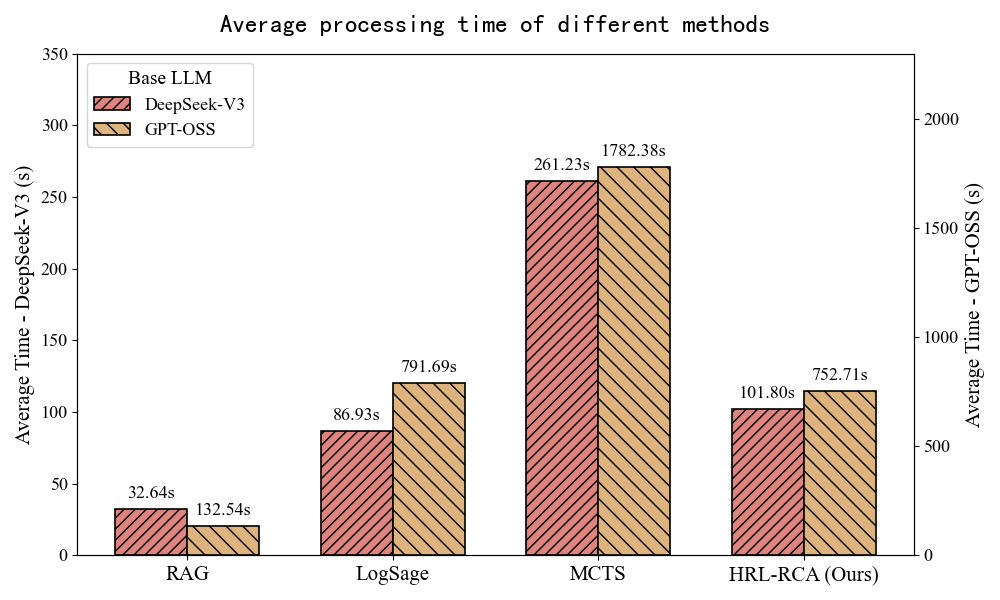
\includegraphics[width=\columnwidth]{pic/HRL-RCA-exp-time.png}
    \caption{Average processing time of different methods}
    \Description{A bar chart showing average runtime in seconds for RAG, LogSage, MCTS, and HRL-RCA, with MCTS being the slowest and HRL-RCA achieving a good balance.}
    \label{fig:efficiency}
\end{figure}

As shown in Figure~\ref{fig:efficiency}, with DeepSeekV3 as the backbone, HRL-RCA achieves an average runtime of 101.80s, reducing processing time by approximately 61.0\% compared with MCTS (261.23s) while remaining comparable to LogSage (86.93s). The naive RAG baseline is the fastest (32.64s) but yields substantially lower accuracy. MCTS incurs the highest latency due to multi-round search-based reasoning, whereas HRL-RCA constrains the candidate space via rule routing, circumventing the overhead of global search while achieving the best overall accuracy and maintaining practical efficiency.

%% ===== Section 5 Conclusion and Future Work =====
\section{Conclusion and Future Work}

This paper addresses build failures in RISC-V package migration and proposes a two-stage root cause analysis framework combining log compression with rule learning. In the first stage, MGSC employs explicit error anchor localization, entity-based long-distance context backtracking, and lightweight semantic compression to preserve high-fidelity evidence chains under strict token budgets, substantially reducing the input size of ultra-long logs. In the second stage, HRL-RCA structures historical repair experience into verifiable rules organized as a rule tree and performs conditional routing during online inference to retrieve rules whose preconditions are satisfied, generating traceable root cause analyses and repair recommendations under explicit evidence constraints.

Experimental results demonstrate that MGSC achieves higher coverage of key evidence than existing compression methods while maintaining stable and controllable output token sizes. HRL-RCA attains a comprehensive diagnostic score of 79.0\%, significantly outperforming naive RAG, multi-path retrieval-augmented methods, and search-based reasoning baselines, while reducing runtime by 61\% relative to MCTS, thereby offering clear advantages in both effectiveness and efficiency. Future work will focus on improving incremental update and deduplication mechanisms for the rule knowledge base, exploring adaptation to additional architectures and build systems, and developing IDE plugins and other developer-facing tools to facilitate adoption in production engineering workflows. Our dataset and tools will be made publicly available upon acceptance to support reproducibility.

\section{Threats to Validity}

\textbf{Internal validity.} The RCA scoring rubric relies on expert judgment. To mitigate subjectivity, each case is independently assessed by three domain experts and the final score is determined by majority vote; the resulting Fleiss' $\kappa$ of 0.72 indicates substantial agreement. The rule-tree construction also involves LLM-based structuring, whose outputs undergo validation by an automated schema checker and a rewrite loop, thereby reducing extraction errors.

\textbf{External validity.} Our dataset is drawn from a single OBS instance focused on RISC-V. Although the 174 cases span five error categories and four build stages, they may not fully represent all failure patterns encountered in other distributions or architectures. We plan to extend the evaluation to additional ecosystems (e.g., Debian, Fedora) and architectures (e.g., LoongArch) in future work.

\textbf{Construct validity.} The composite score equally weights four sub-dimensions. Different weighting schemes could shift relative rankings. We adopt equal weights for simplicity and report per-dimension scores in Table~\ref{tab:hrl-results} and Figure~\ref{fig:sub-scores} to allow readers to assess each dimension independently.

%%
%% Acknowledgments (hidden for submission)
%%
%\begin{acks}
%This work was supported in part by projects of the Institute of Software, Chinese Academy of Sciences, among others.
%\end{acks}

%%
%% Bibliography
%%
\bibliographystyle{ACM-Reference-Format}
\bibliography{reference}

\end{document}